% You should title the file with a .tex extension (hw1.tex, for example)
\documentclass[11pt]{article}

\usepackage{amsmath}
\usepackage{amssymb}
\usepackage{fancyhdr}
\usepackage{listings}
\usepackage{color}
\usepackage{graphicx}
\graphicspath{ {images/} }
\usepackage{hyperref}
\usepackage{mathtools}

\definecolor{dkgreen}{rgb}{0,0.6,0}
\definecolor{gray}{rgb}{0.5,0.5,0.5}
\definecolor{mauve}{rgb}{0.58,0,0.82}

\lstset{frame=tb,
  language=Java,
  aboveskip=3mm,
  belowskip=3mm,
  showstringspaces=false,
  columns=flexible,
  basicstyle={\small\ttfamily},
  numbers=none,
  numberstyle=\tiny\color{gray},
  keywordstyle=\color{blue},
  commentstyle=\color{dkgreen},
  stringstyle=\color{mauve},
  breaklines=true,
  breakatwhitespace=true,
  tabsize=3
}

\oddsidemargin0cm
\topmargin-2cm     %I recommend adding these three lines to increase the 
\textwidth16.5cm   %amount of usable space on the page (and save trees)
\textheight23.5cm  

\newcommand{\question}[2] {\vspace{.25in} \hrule\vspace{0.5em}
\noindent{\bf #1: #2} \vspace{0.5em}
\hrule \vspace{.10in}}
\renewcommand{\part}[1] {\vspace{.10in} {\bf (#1)}}

\newcommand{\myname}{Chang-Hyun Mungai}
\newcommand{\myhwnum}{Structural Notes}

\setlength{\parindent}{0pt}
\setlength{\parskip}{5pt plus 1pt}
 
\pagestyle{fancyplain}
\lhead{\fancyplain{}{\textbf{\myhwnum}}}      % Note the different brackets!

\begin{document}

\medskip                        % Skip a "medium" amount of space
                                % (latex determines what medium is)
                                % Also try: \bigskip, \littleskip

\thispagestyle{plain}
\begin{center}                  % Center the following lines
{\Large Structural} \\
\end{center}

\question{General}

\begin{itemize}
   \item ease the design by identifying a simple way to realize relationships between entities
   \item about class and object composition
   \item use inheritance to compose interfaces
   \item define ways to compose objects to obtain new functionality
\end{itemize}

\question{Adapter}

\begin{itemize}
   \item Definition/Use

  \begin{itemize}
     \item 'adapts' one interface for a class into one that a client expects
     \item used when a client class has to call an incompatible provider class
     \item an "off the shelf" component offers compelling functionality but its "view of the world" is not compatible
     \item wrap an existing class with a new interface
  \end{itemize}

   \item Structure

  \begin{itemize}
     \item 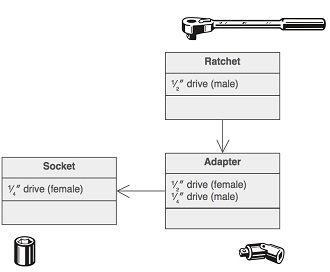
\includegraphics{adapter_example}
     \item 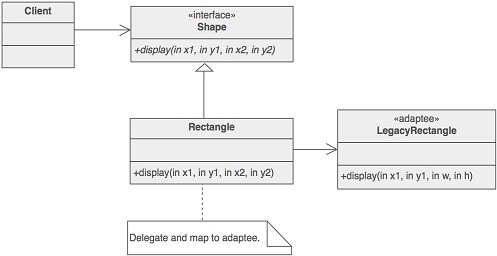
\includegraphics{adapter_example2}
  \end{itemize}

   \item Notes

  \begin{itemize}
     \item put the adapter term in the name of the adapter class to indicate the use of the pattern to the other developers
  \end{itemize}

\end{itemize}

\question{Bridge}

\begin{itemize}
   \item Definition/Use

  \begin{itemize}
     \item decouple an abstraction from its implementation so that the two can vary independently
     \item useful when a code often changes for an implementation as well as for a use of code
     \item decouple an abstraction from its implementation so that the two can vary independently
  \end{itemize}

   \item Structure

  \begin{itemize}
     \item 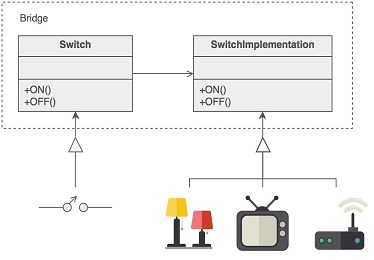
\includegraphics{bridge_example}
  \end{itemize}

   \item Notes

  \begin{itemize}
     \item design the separation of concerns: what does the client want, and what do the platforms provide
  \end{itemize}

\end{itemize}

\question{Composite}

\begin{itemize}
   \item Definition/Use

  \begin{itemize}
     \item a tree structure of objects where every object has the same interface
     \item application needs to manipulate a hierarchical collection of "primitive"(leaf) and "composite" objects
  \end{itemize}

   \item Structure

  \begin{itemize}
     \item 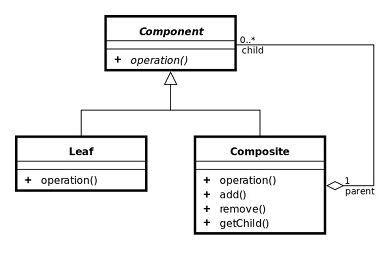
\includegraphics{composite_uml_class_diagram}
     \item 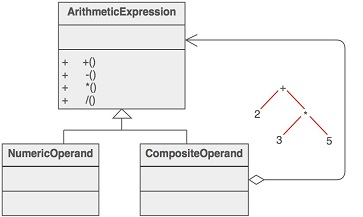
\includegraphics{composite_example}
  \end{itemize}

   \item Examples

  \begin{itemize}
     \item GUI, widgets organized in a tree and operations (resize, repainting) on all widgets processed using pattern
  \end{itemize}

   \item Notes

  \begin{itemize}
     \item consider the heuristic, "containers that contain containees, each of which could be a container"
  \end{itemize}

\end{itemize}

\question{Decorator (Wrapper)}

\begin{itemize}
   \item Definition/Use

  \begin{itemize}
     \item add additional functionality to a class at runtime where subclassing would result in an exponential rise of new classes
     \item client-specified embellishment of a core object by recursively wrapping it
  \end{itemize}

   \item Structure

  \begin{itemize}
     \item 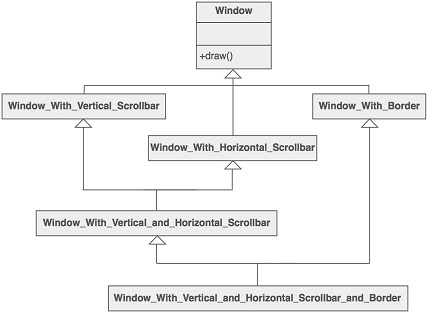
\includegraphics{decorator}

    \begin{itemize}
       \item 
\begin{lstlisting}
Widget* aWidget = new BorderDecorator(
  new HorizontalScrollBarDecorator(
    new VerticalScrollBarDecorator(
      new Window( 80, 24 ))));
aWidget->draw();
\end{lstlisting}
    \end{itemize}

  \end{itemize}

   \item Notes

  \begin{itemize}
     \item ensure the context is: a single core (or non-optional) component, several optional embellishments or wrappers, and an interface that is common to all
  \end{itemize}

\end{itemize}

\question{Farcade}

\begin{itemize}
   \item Definition/Use

  \begin{itemize}
     \item create a simplified interface of an existing interface to ease usage for common tasks
     \item hides the complexities of the system and provides an interface to the client from where the client can access the system
  \end{itemize}

   \item Structure

  \begin{itemize}
     \item 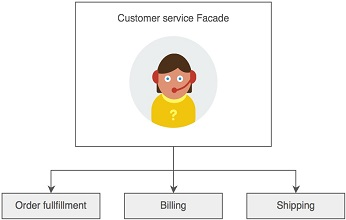
\includegraphics{facade_example}
  \end{itemize}

   \item Notes

  \begin{itemize}
     \item often singletons because only one facade object is required
     \item client uses (is coupled to) the facade only
  \end{itemize}

\end{itemize}

\question{Flyweight}

\begin{itemize}
   \item Definition/Use

  \begin{itemize}
     \item a large quantity of objects share a common properties object to save space
     \item each "flyweight" object is divided into two pieces

    \begin{itemize}
       \item the state-dependent (extrinsic) part: stored or computed by client objects, and passed to the Flyweight when its operations are invoked
       \item the state-independent (intrinsic) part: stored (shared) in the Flyweight object
    \end{itemize}

  \end{itemize}

   \item Example

  \begin{itemize}
     \item in video games, it is usual that you have to display the same sprite (i.e. an image of an item of the game) several times

    \begin{itemize}
       \item it would highly use the CPU and the memory if each sprite was a different object
       \item so the sprite is created once and then is rendered at different locations in the screen
       \item this problem can be solved using the flyweight pattern
       \item the object that renders the sprite is a flyweight
    \end{itemize}

  \end{itemize}

\end{itemize}

\question{Proxy}

\begin{itemize}
   \item Definition/Use

  \begin{itemize}
     \item a class functioning as an interface to another thing
     \item provide a surrogate or placeholder for another object to control access to it
  \end{itemize}

   \item Structure

  \begin{itemize}
     \item 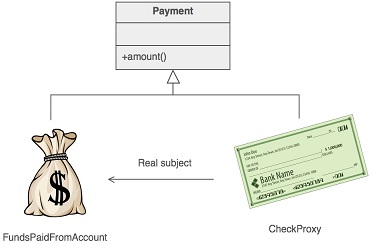
\includegraphics{proxy_example}
  \end{itemize}

   \item Example

  \begin{itemize}
     \item ProxyImage and RealImage
  \end{itemize}

\end{itemize}

\question{Comparison}

\begin{itemize}
   \item adapter makes things work after they're designed, bridge makes them work before they are
   \item composite and decorator have similar structure diagrams, reflecting the fact that both rely on recursive composition to organize an open-ended number of objects
   \item decorator and proxy have different purposes but similar structures
\end{itemize}

\end{document}

